\documentclass[11pt,letterpaper]{article}
\usepackage{graphicx, geometry, amsmath, amssymb, booktabs, xcolor, listings}
\usepackage[numbers,sort&compress]{natbib}
\usepackage{hyperref}
\usepackage{url}
\geometry{margin=1in}
\hypersetup{colorlinks=true, linkcolor=black, citecolor=black, urlcolor=black}

\title{Extreme Value Analysis of Maximum Dependency Distances:\\Framework, Validation, and Association with Word-Order Entropy\\Across 238 Universal Dependencies Treebanks}

\author{~}
\date{~}

\begin{document}
\maketitle

\begin{abstract}
Two decades of dependency length minimization research have focused on mean dependency distance, leaving the tail behavior of sentence-level maxima unexplored. We fit Generalized Extreme Value (GEV) distributions to per-sentence maximum dependency distances across 918 bin--treebank combinations from 238 Universal Dependencies treebanks spanning 122 languages, extracting the shape parameter $\xi$ as an index of tail-constraint severity. GEV outperforms lognormal and gamma alternatives by AIC in 95.2\% of combinations, though only 28.2\% pass absolute Anderson-Darling/Kolmogorov-Smirnov goodness-of-fit tests --- a tension we report transparently. Among treebank pairs with similar mean dependency distances, 46.2\% differ meaningfully in $\xi$, demonstrating that the framework captures cross-linguistic variation invisible to existing approaches. Mixed-effects regression with 26 language-family random intercepts identifies word-order entropy as associated with $\xi$ ($\beta = 0.084$, $p_{\text{FDR}} = 0.0007$), but this association vanishes when analysis is restricted to the 28.2\% of combinations with adequate absolute fit ($p = 0.93$). Mediation analysis reveals a pattern statistically consistent with --- but not proving --- a structural-distributional interpretation: the indirect path through word-order entropy is significant while the direct morphology-to-$\xi$ path is not, though opposing indirect and direct effects yield a near-zero total effect. We contribute three validation protocols --- bound-awareness simulation, dual-track normalization, and super-block sensitivity analysis --- that address fundamental challenges of applying extreme value theory to bounded linguistic data.
\end{abstract}

\section{Introduction}

The principle of dependency length minimization (DLM) --- that languages tend to place syntactically related words close together in linear order --- is among the most robust quantitative universals in linguistics \cite{Futrell2015, Liu2017}. Futrell, Mahowald, and Gibson demonstrated DLM across 37 languages from 10 families, finding significance at $p < 0.0001$ for every language under free word-order baselines \cite{Futrell2015}. Subsequent work extended DLM analysis to 54 languages, revealing that word-order typology interacts with the magnitude of minimization: SOV languages show weaker DLM than SVO languages \cite{Yadav2020, Yadav2022}. Li and Liu examined 55 languages across 11 families, finding that morphological richness correlates more strongly with syntactic directionality than with word-order entropy \cite{Li2025}. Petrini and Ferrer-i-Cancho fitted two-regime exponential models to dependency distance distributions in 20 languages, identifying a universal breakpoint at 4--5 words \cite{Petrini2025}.

All of these studies analyze the central tendency or full distribution of \emph{all} dependency distances. The longest dependency in a sentence, however, is a key predictor of processing difficulty --- the point where working memory is most severely taxed \cite{Liu2017, Liu2008}. Experimental evidence confirms that per-sentence maximum dependency distance (max\_DD) correlates with disfluencies and comprehension difficulty beyond what mean dependency distance captures \cite{Liu2017}, though intervener complexity and surprisal also contribute to processing load \cite{Yadav2022}. Information about how sharply constrained these extremes are --- whether a language permits occasional very long dependencies or imposes a rigid upper ceiling --- is mathematically inaccessible from any analysis restricted to means, sums, or two-regime models of all dependency distances.

This gap motivates a methodological transfer from environmental statistics and structural engineering, where the Generalized Extreme Value (GEV) distribution is the standard tool for characterizing extreme events such as 100-year floods and maximum wind speeds \cite{Coles2001, Hosking1997}. The key insight from reliability engineering is that the \emph{nature} of a system's behavior under extreme loads --- whether bounded sharply or decaying gradually --- is encoded in the GEV shape parameter $\xi$, and this distinction carries qualitatively different information from the system's average behavior.

Applying EVT to linguistic data raises two challenges that demand transparency. First, for sentences of length $n$, max\_DD is theoretically bounded in $[1, n{-}1]$, whereas classical EVT assumes effectively unbounded distributions \cite{Coles2001}. Second, sentences contain only 9--19 dependency arcs for lengths 10--20, far fewer observations per block than the annual maxima (365+ daily values) standard in hydrology. Addressing both concerns requires validation protocols imported from flood-frequency analysis \cite{Coles2001, Hosking1997} --- but as we show, these validations yield mixed results that substantially qualify the interpretability of $\xi$ as a tail-shape parameter.

We fit GEV distributions to 918 qualifying bin--treebank combinations from 238 Universal Dependencies treebanks and find that $\xi$ captures cross-linguistic variation invisible to mean dependency distance: 46.2\% of treebank pairs with similar mean DD differ meaningfully in $\xi$. Mixed-effects regression identifies word-order entropy as a significant predictor of $\xi$ ($\beta = 0.084$, $p_{\text{FDR}} = 0.0007$), but sensitivity analysis reveals that this association vanishes when analysis is restricted to combinations with adequate absolute goodness-of-fit ($p = 0.93$), and formal ordinal validity testing of $\xi$ produces mixed results (1 of 4 tests pass). Mediation analysis reveals a pattern statistically consistent with the structural-distributional interpretation that morphological richness influences $\xi$ through word-order flexibility, though the near-zero total effect and opposing indirect and direct paths warrant cautious interpretation. The framework's primary contribution is methodological: three validation protocols that establish when and how EVT can be applied to bounded linguistic data. An overview of the complete framework is shown in Figure~\ref{fig:framework}.

\subsection{Summary of Contributions}

This paper makes three contributions:

\begin{itemize}
  \item \textbf{An EVT framework with extensive validation.} We fit GEV distributions to per-sentence max\_DD across 918 bin--treebank combinations from 238 UD treebanks, extracting $\xi$ with bootstrap confidence intervals. Three validation protocols --- bound-awareness simulation (${\sim}3$ million random projective linearizations), dual-track normalization (raw vs.\ normalized, $\rho = 0.9997$), and super-block sensitivity analysis --- establish the framework's strengths and limitations before typological interpretation (Section~\ref{sec:methods}).
  \item \textbf{Transparent reporting of both favorable and unfavorable validation results.} GEV is AIC-best in 95.2\% of combinations but passes absolute goodness-of-fit tests in only 28.2\%. Super-block $\xi$ correlations are negative ($\rho = -0.39$ to $-0.55$), though non-parametric quantile rankings show near-perfect preservation ($\rho_{p95} = 0.986$). The word-order entropy association with $\xi$ survives family-audit correction, annotation-quality filtering, and leave-one-family-out cross-validation, but vanishes under goodness-of-fit restriction (Section~\ref{sec:results}).
  \item \textbf{A qualified test of structural vs.\ cognitive explanations.} Cross-sectional mediation analysis reveals opposing indirect and direct paths with a near-zero total effect, statistically consistent with the structural-distributional interpretation but insufficient to establish causal ordering. The reverse mediation model is distinguishable, providing one asymmetric piece of evidence (Section~\ref{sec:discussion}).
\end{itemize}

\begin{figure}[!htbp]
  \centering
  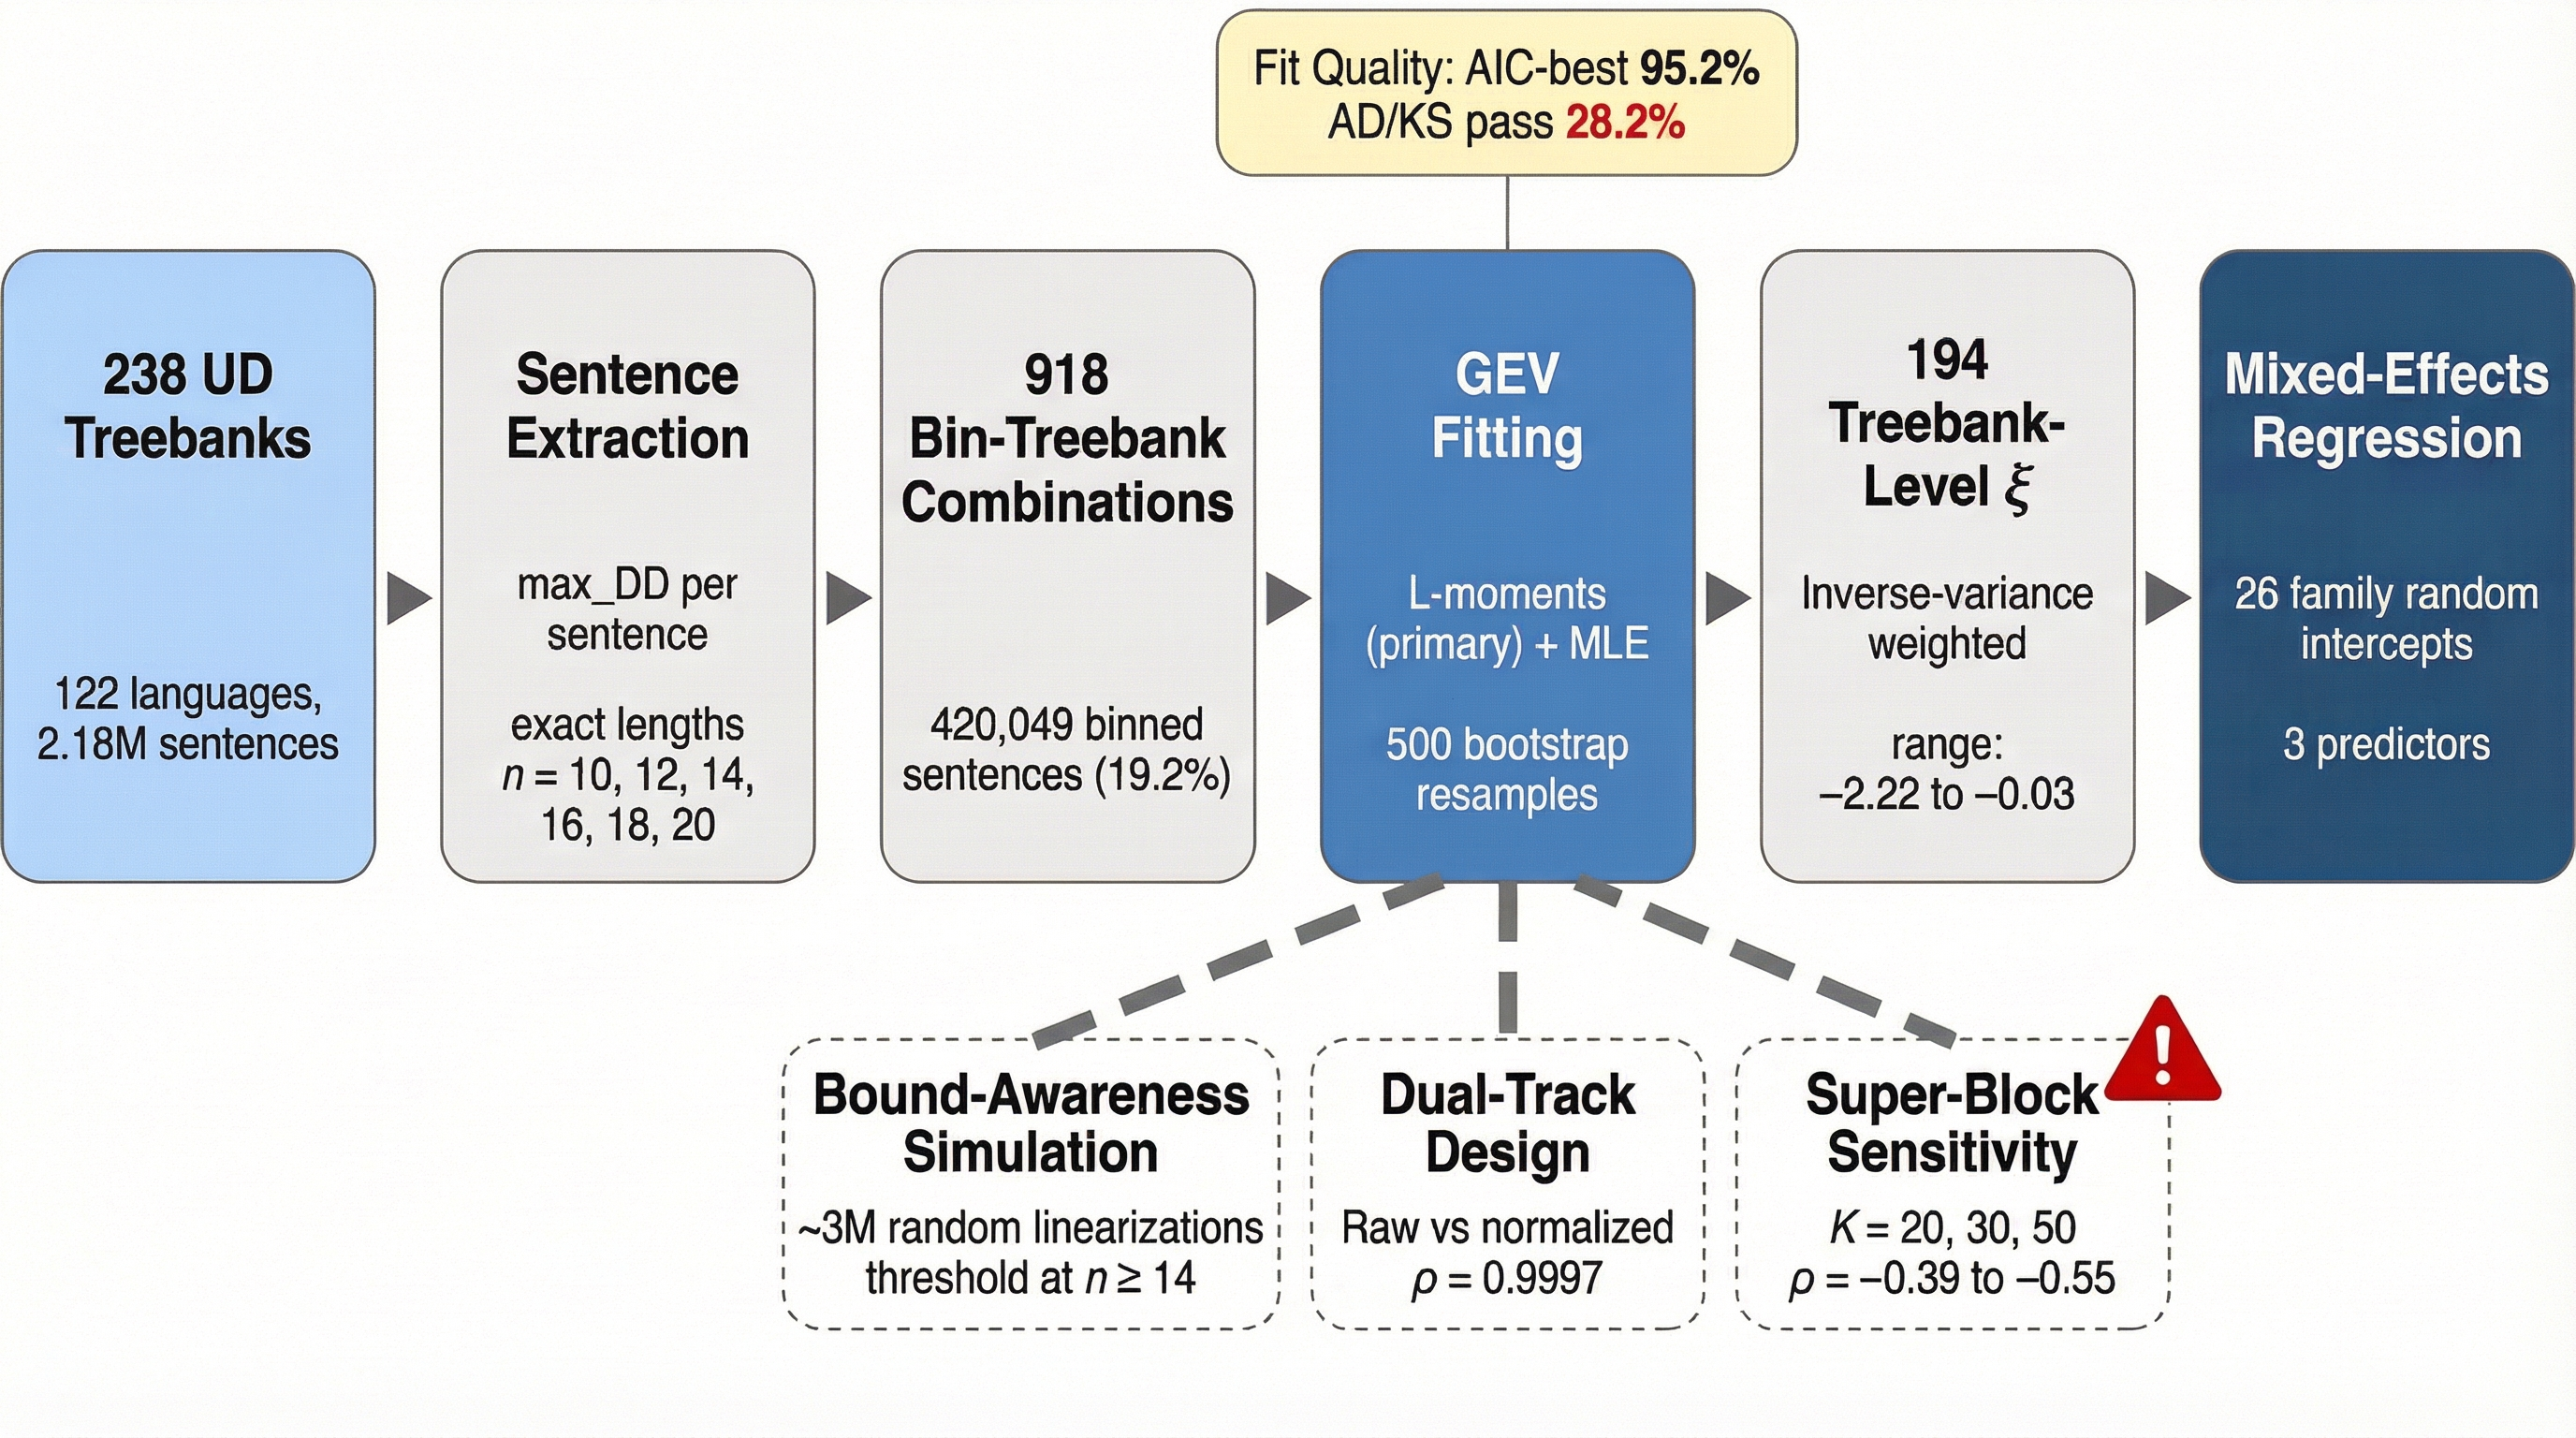
\includegraphics[width=0.92\textwidth,keepaspectratio]{figures/fig1_v0.png}
  \caption{Overview of the Extreme Value Theory framework for characterizing tail behavior of maximum dependency distances. The pipeline extracts per-sentence max\_DD from 238 UD treebanks, bins sentences by exact length ($n \in \{10, 12, 14, 16, 18, 20\}$), fits GEV distributions to extract $\xi$, and relates treebank-level $\xi$ to typological features via mixed-effects regression. Three validation protocols (bound-awareness simulation, dual-track normalization, super-block sensitivity) assess framework applicability before typological interpretation.}
  \label{fig:framework}
\end{figure}

\section{Related Work}\label{sec:related}

\subsection{Dependency Distance Minimization}

The DLM literature spans two decades, beginning with systematic quantitative analyses by Liu \cite{Liu2017, Liu2010} and culminating in Futrell et al.'s landmark demonstration across 37 languages \cite{Futrell2015}. The key finding is that observed mean dependency distances are significantly shorter than random projective baselines in virtually all languages studied, consistent with pressure to minimize working-memory burden during incremental parsing. Cross-linguistic variation in DLM magnitude has been linked to word-order typology: head-final languages show less minimization than head-initial languages, hypothetically because case marking reduces reliance on linear proximity \cite{Futrell2015}. Yadav et al.\ confirmed this pattern across 38 languages and further showed that dependency distances are determined by default word order \cite{Yadav2020}. Their reappraisal across 54 languages showed that the DLM effect persists after controlling for intervener complexity \cite{Yadav2022}, suggesting that both word-count distance and syntactic interveners contribute to processing load. Alemany-Puig and Ferrer-i-Cancho provided efficient algorithms for computing expected edge lengths in random projective linearizations \cite{AlemanyPuig2022}, enabling large-scale baseline comparisons.

\subsection{Distribution of Dependency Distances}

Petrini and Ferrer-i-Cancho modeled the full distribution of all dependency distances across 20 Parallel UD treebanks \cite{Petrini2025}. Their two-regime exponential model, with a breakpoint averaging 4--5 words, suggests a universal cognitive processing threshold. Crucially, their analysis aggregates all dependency distances within a corpus, not per-sentence maxima. The GEV framework operates on a fundamentally different statistical object: block maxima (per-sentence max\_DD) rather than pooled observations, extracting tail-shape information invisible to any analysis of the full distribution or its central tendency.

\subsection{Typological Correlates}

Li and Liu examined interactions among morphological richness, word-order entropy, and syntactic directionality across 55 languages using 80 UD treebanks \cite{Li2025}. They found that morphological richness correlates with syntactic directionality (head-finality) but only weakly with word-order entropy after statistical correction. Levshina developed token-based entropy measures of word-order flexibility from UD corpora, showing that word-order entropy correlates with morphological overlap between grammatical roles \cite{Levshina2019}. The present work assigns Levshina's word-order entropy a novel analytical role as the predictor of GEV tail-constraint severity and as the mediator variable in a formal test distinguishing structural-distributional from cognitive explanations for $\xi$ variation.

\subsection{Extreme Value Theory}

The GEV distribution and block maxima method are standard in hydrology \cite{Coles2001, Hosking1997}, structural engineering \cite{Coles2001}, and climate science, where they characterize 100-year floods, design wind speeds, and temperature extremes. Hosking introduced L-moments estimation \cite{Hosking1990}, which provides more robust GEV parameter estimates than maximum likelihood for moderate sample sizes ($n < 500$) \cite{Hosking1997}. Laio developed modified Anderson-Darling and Cram\'er--von Mises goodness-of-fit tests for extreme value distributions with unknown parameters \cite{Laio2004}, providing the absolute fit assessment used in the present work. To our knowledge, EVT has not previously been applied to dependency distance analysis or syntactic complexity measures.

\subsection{Mediation Analysis Methodology}

The Preacher-Hayes bootstrap method \cite{Preacher2015} is widely used for testing indirect effects in psychology, but extensive methodological literature warns that mediation analysis on cross-sectional data cannot establish causal ordering \cite{Maxwell2007}. Maxwell and Cole demonstrated that cross-sectional mediation typically generates substantially biased estimates of longitudinal mediation parameters even under ideal conditions when mediation is complete \cite{Maxwell2007}. Cross-sectional mediation establishes statistical consistency with a proposed causal model but cannot distinguish the proposed model from alternative orderings or unobserved confounds \cite{Preacher2015, Maxwell2007}. The present work adopts the more cautious interpretation standard from this literature.

\section{Methods}\label{sec:methods}

\subsection{Data Source and Extraction}

We extract sentence-level dependency distance data from the commul/universal\_dependencies HuggingFace dataset, which provides UD v2.17 treebanks in Parquet format \cite{deMarneffe2021}. For each sentence, dependency distances are computed as $|position(\text{dependent}) - position(\text{head})|$ for all syntactic arcs, and the sentence-level maximum (max\_DD) is extracted\footnote{Code: \url{https://github.com/AMGrobelnik/ai-invention-42dac1-word-order-entropy-predicts-ordinal-tail/tree/main/dataset_iter1_ud_sentence_max}}. Both raw max\_DD and normalized max\_DD/$(n{-}1)$ are recorded.

Treebanks with fewer than 500 total sentences are excluded. Sentences are grouped into non-overlapping fixed-length bins at exactly $n \in \{10, 12, 14, 16, 18, 20\}$. Bin--treebank combinations with fewer than 50 sentences are excluded from GEV fitting but retained for descriptive statistics. The exact-length binning retains 420,049 of 2,181,479 total sentences (19.2\%); a representativeness analysis confirms that genre and modality distributions in the binned subset do not differ systematically from the full corpus\footnote{Code: \url{https://github.com/AMGrobelnik/ai-invention-42dac1-word-order-entropy-predicts-ordinal-tail/tree/main/experiment_iter2_data_quality_va}}.

\subsection{Typological Feature Computation}

Three typological features are computed for each treebank from the UD annotations:

\textbf{Morphological richness} is the mean number of non-empty morphological features per token, computed from the UD feats column. Values range from 0.0 (Korean ko\_kaist, Japanese ja\_gsd) to 4.51, with a mean of 1.73 across the 238 qualifying treebanks.

\textbf{Head-direction ratio} is the proportion of dependency arcs where the head precedes the dependent, excluding root arcs. Values range from 0.18 (Turkish) to 0.79 (Guajajara), with a mean of 0.44.

\textbf{Word-order entropy} follows Levshina \cite{Levshina2019}: for each dependency relation type with at least 20 token occurrences, the binary Shannon entropy $H = -p\log_2 p - (1{-}p)\log_2(1{-}p)$ is computed, where $p$ is the proportion of head-before-dependent instances. Relation-level entropies are averaged, weighted by token frequency. Punctuation and root relations are excluded. A sensitivity analysis confirms near-perfect rank stability ($\rho = 0.9999$) between frequency thresholds of 10 and 20. Word-order entropy ranges from 0.01 (rigid order) to 0.77 (free order), with a mean of 0.34.

\subsection{Grambank Cross-Validation}

To guard against annotation artifacts in corpus-based morphological richness, we cross-validate against Grambank v1.0.3 \cite{Skirgard2023}, an independently constructed typological database. We identify 87 morphology-relevant features using the authoritative domain classification from grambank-analysed (nominal, verbal, and pronoun domains crossed with argument marking, TAME, number, and class groupings)\footnote{Code: \url{https://github.com/AMGrobelnik/ai-invention-42dac1-word-order-entropy-predicts-ordinal-tail/tree/main/dataset_iter1_grambank_morpho}}. For each language, a morphological complexity index is computed as the proportion of present features among coded ones, with a minimum threshold of 15 coded features. Languages are mapped to UD treebanks via Glottocode-to-ISO through Glottolog \cite{Hammarstrom2024}, with macro-language resolution (e.g., arb $\rightarrow$ ara, cmn $\rightarrow$ zho).

The Grambank mapping identifies 178 treebank--Grambank pairings. The correlation between corpus-based UD morphological richness and the Grambank index yields Spearman $\rho = 0.34$ ($p < 0.001$) and Pearson $r = 0.42$ ($p < 0.001$)\footnote{Code: \url{https://github.com/AMGrobelnik/ai-invention-42dac1-word-order-entropy-predicts-ordinal-tail/tree/main/experiment_iter2_gev_tail_constr}}. This moderate positive correlation confirms that the two measures capture related but non-identical aspects of morphological complexity. Annotation completeness (the proportion of tokens with non-empty feats fields) correlates strongly with morphological richness ($\rho = 0.79$), indicating that treebanks with incomplete morphological annotation yield artificially low richness scores. The downstream consequences of this confound are addressed through a sensitivity analysis restricting to well-annotated treebanks (Section~\ref{sec:sensitivity}).

\subsection{Language-Family Audit}

All 238 language-to-family mappings were audited against Glottolog \cite{Hammarstrom2024} and UD metadata\footnote{Code: \url{https://github.com/AMGrobelnik/ai-invention-42dac1-word-order-entropy-predicts-ordinal-tail/tree/main/evaluation_iter3_family_audit_an}}. One misclassification was identified and corrected: Afrikaans (af\_afribooms), originally classified as Afro-Asiatic, was reassigned to Indo-European (Germanic). The total number of language families remains 26 after correction. The corrected regression results are reported throughout; the correction has negligible impact on the entropy coefficient ($\Delta\beta = 0.0005$, confidence intervals fully overlapping).

\subsection{GEV Framework}

\subsubsection{GEV as a Flexible Parametric Family}

The Generalized Extreme Value distribution with CDF
\begin{equation}\label{eq:gev}
G(x; \mu, \sigma, \xi) = \exp\left\{-\left[1 + \xi\left(\frac{x - \mu}{\sigma}\right)\right]^{-1/\xi}\right\}
\end{equation}
where $\mu$ is the location, $\sigma > 0$ the scale, and $\xi$ the shape parameter, unifies three tail regimes: $\xi < 0$ (Weibull, bounded upper tail), $\xi = 0$ (Gumbel, exponential tail decay), and $\xi > 0$ (Fr\'echet, heavy power-law tail) \cite{Coles2001}.

The classical Fisher--Tippett--Gnedenko theorem guarantees GEV convergence for maxima over large block sizes, but individual sentences contain only 9--19 dependency arcs for lengths 10--20. We therefore frame GEV not as an asymptotic convergence result but as a flexible three-parameter parametric family for describing the distribution of per-sentence max\_DD. Three validation protocols empirically assess the adequacy and interpretability of this pragmatic use.

\subsubsection{Estimation}

GEV parameters are estimated using both L-moments estimation (via lmoments3) \cite{Hosking1990} and maximum likelihood estimation (via scipy.stats.genextreme). A critical sign convention must be observed: both packages parameterize the GEV with $c = -\xi$, so all fitted $c$ values are negated before interpretation\footnote{Code: \url{https://github.com/AMGrobelnik/ai-invention-42dac1-word-order-entropy-predicts-ordinal-tail/tree/main/research_iter1_gev_fitting_met}}. L-moments estimation is preferred as the primary method for bin--treebank combinations with fewer than 500 sentences, as it produces lower RMSE for the shape parameter than MLE in small samples \cite{Hosking1990}. Bootstrap confidence intervals (500 resamples) are computed for all $\xi$ estimates.

\subsubsection{Bound-Awareness Validation}

Since max\_DD is bounded in $[1, n{-}1]$, a simulation protocol validates GEV applicability before typological interpretation. For each target sentence length $n \in \{10, 12, 14, 16, 18, 20\}$, dependency trees from 10 typologically diverse treebanks are randomly linearized maintaining projectivity (following Futrell et al.\ \cite{Futrell2015} and Alemany-Puig and Ferrer-i-Cancho \cite{AlemanyPuig2022}), generating approximately 3 million random linearizations\footnote{Code: \url{https://github.com/AMGrobelnik/ai-invention-42dac1-word-order-entropy-predicts-ordinal-tail/tree/main/experiment_iter2_bound_awareness}}. GEV is fitted to the resulting null max\_DD distributions via L-moments. The range of $\xi$ estimates across treebanks under this null model determines whether the raw track supports meaningful variation at each length: if the null $\xi$ range exceeds 0.25, cross-treebank $\xi$ differences in real data can reflect genuine structural differences rather than bound proximity alone.

\subsubsection{Dual-Track Design}

The primary analysis uses raw max\_DD within fixed-length bins, where the theoretical upper bound $n{-}1$ may be distant from the practical data range. The sensitivity analysis uses normalized max\_DD/$(n{-}1)$, mapping values to $(0, 1]$ and restricting interpretation to $\xi$-magnitude gradients within the Weibull domain. Agreement between tracks is assessed via Spearman $\rho$ on treebank $\xi$ rankings.

\subsubsection{Fit Quality Assessment: Relative and Absolute}

GEV adequacy is assessed using two complementary criteria. Relative fit quality compares GEV against lognormal and gamma alternatives using AIC/BIC model selection \cite{Burnham2004}. Absolute fit quality uses Anderson-Darling/Kolmogorov-Smirnov goodness-of-fit tests \cite{Laio2004} to assess whether the GEV parametric form adequately describes each bin's max\_DD distribution. Both metrics are reported transparently, as relative superiority does not imply absolute adequacy.

\subsubsection{Super-Block Sensitivity Analysis}

To assess whether single-sentence $\xi$ estimates are consistent with estimates from larger blocks where EVT convergence is better justified, super-blocks of $K = 20$, 30, and 50 same-length sentences are constructed, taking the maximum max\_DD across each block, and GEV is fitted to the resulting super-block maxima\footnote{Code: \url{https://github.com/AMGrobelnik/ai-invention-42dac1-word-order-entropy-predicts-ordinal-tail/tree/main/experiment_iter2_super_block_gev}}. $\xi$ rankings from super-block fits are compared with single-sentence estimates via Spearman $\rho$.

\subsection{Statistical Analysis}

\subsubsection{Mixed-Effects Regression}

Treebank-level $\xi$ (aggregated across bins via inverse-variance weighting) is regressed on morphological richness, head-direction ratio, and word-order entropy (all standardized) using a mixed-effects linear model with language-family random intercepts (26 families after audit correction). Variance inflation factors (VIF $< 5$ required), partial correlations, and FDR correction (Benjamini--Hochberg) across predictors are reported.

\subsubsection{Mediation Analysis}

A formal mediation analysis using the Preacher--Hayes bootstrap method (5,000 resamples) \cite{Preacher2015} tests whether word-order entropy mediates the morphology $\rightarrow \xi$ pathway. Following the recommendations of Maxwell and Cole \cite{Maxwell2007} and Preacher \cite{Preacher2015} regarding cross-sectional mediation, results are interpreted as establishing statistical consistency with a proposed causal model, not as evidence for a specific causal ordering.

\subsubsection{Sensitivity Analyses}\label{sec:sensitivity_methods}

Four sensitivity tracks are conducted: (1) corrected regression after family audit; (2) restriction to bin--treebank combinations passing absolute goodness-of-fit tests; (3) restriction to treebanks with feature-annotation completeness $> 0.5$; (4) leave-one-family-out cross-validation across all 26 families. A reverse mediation analysis (entropy $\rightarrow$ morphology $\rightarrow \xi$) and a formal ordinal validity evaluation of $\xi$ complement the primary sensitivity tracks\footnote{Code: \url{https://github.com/AMGrobelnik/ai-invention-42dac1-word-order-entropy-predicts-ordinal-tail/tree/main/evaluation_iter3_ordinal_validit}}.

\section{Results}\label{sec:results}

\subsection{GEV Model Fit Quality: Relative and Absolute}

GEV distributions were fitted to all 918 qualifying bin--treebank combinations using both L-moments and MLE, with L-moments as primary. GEV is AIC-best in 95.2\% of combinations compared to lognormal and gamma alternatives, substantially exceeding the 70\% relative adequacy threshold. Mean absolute difference between MLE and L-moments $\xi$ estimates is 0.029, indicating good method agreement.

However, only 28.2\% of combinations (259 of 918) pass absolute Anderson-Darling/Kolmogorov-Smirnov goodness-of-fit tests. Being the best-fitting distribution among three candidates is a relative comparison that does not establish absolute adequacy. The low absolute pass rate means that individual $\xi$ magnitudes should be interpreted cautiously --- the GEV parametric form does not accurately describe the max\_DD distribution in the majority of bins, even though no standard alternative provides a better fit. The implications of this tension for the typological results are examined in Section~\ref{sec:sensitivity}.

Shape parameter $\xi$ is aggregated per treebank via inverse-variance weighting across qualifying bins, yielding estimates for 194 treebanks. All 194 treebank-level $\xi$ values fall in the Weibull domain ($\xi < 0$), ranging from $-2.22$ to $-0.03$ with mean $-0.43$ (SD $= 0.23$, median $= -0.42$). The distribution comprises: 27.8\% strongly Weibull ($\xi < -0.5$), 59.3\% moderately Weibull ($-0.5 \leq \xi < -0.2$), and 12.9\% weakly Weibull ($-0.2 \leq \xi < 0$). No treebank falls in the Gumbel or Fr\'echet domains. The full distribution is shown in Figure~\ref{fig:xi_dist}.

\begin{figure}[!htbp]
  \centering
  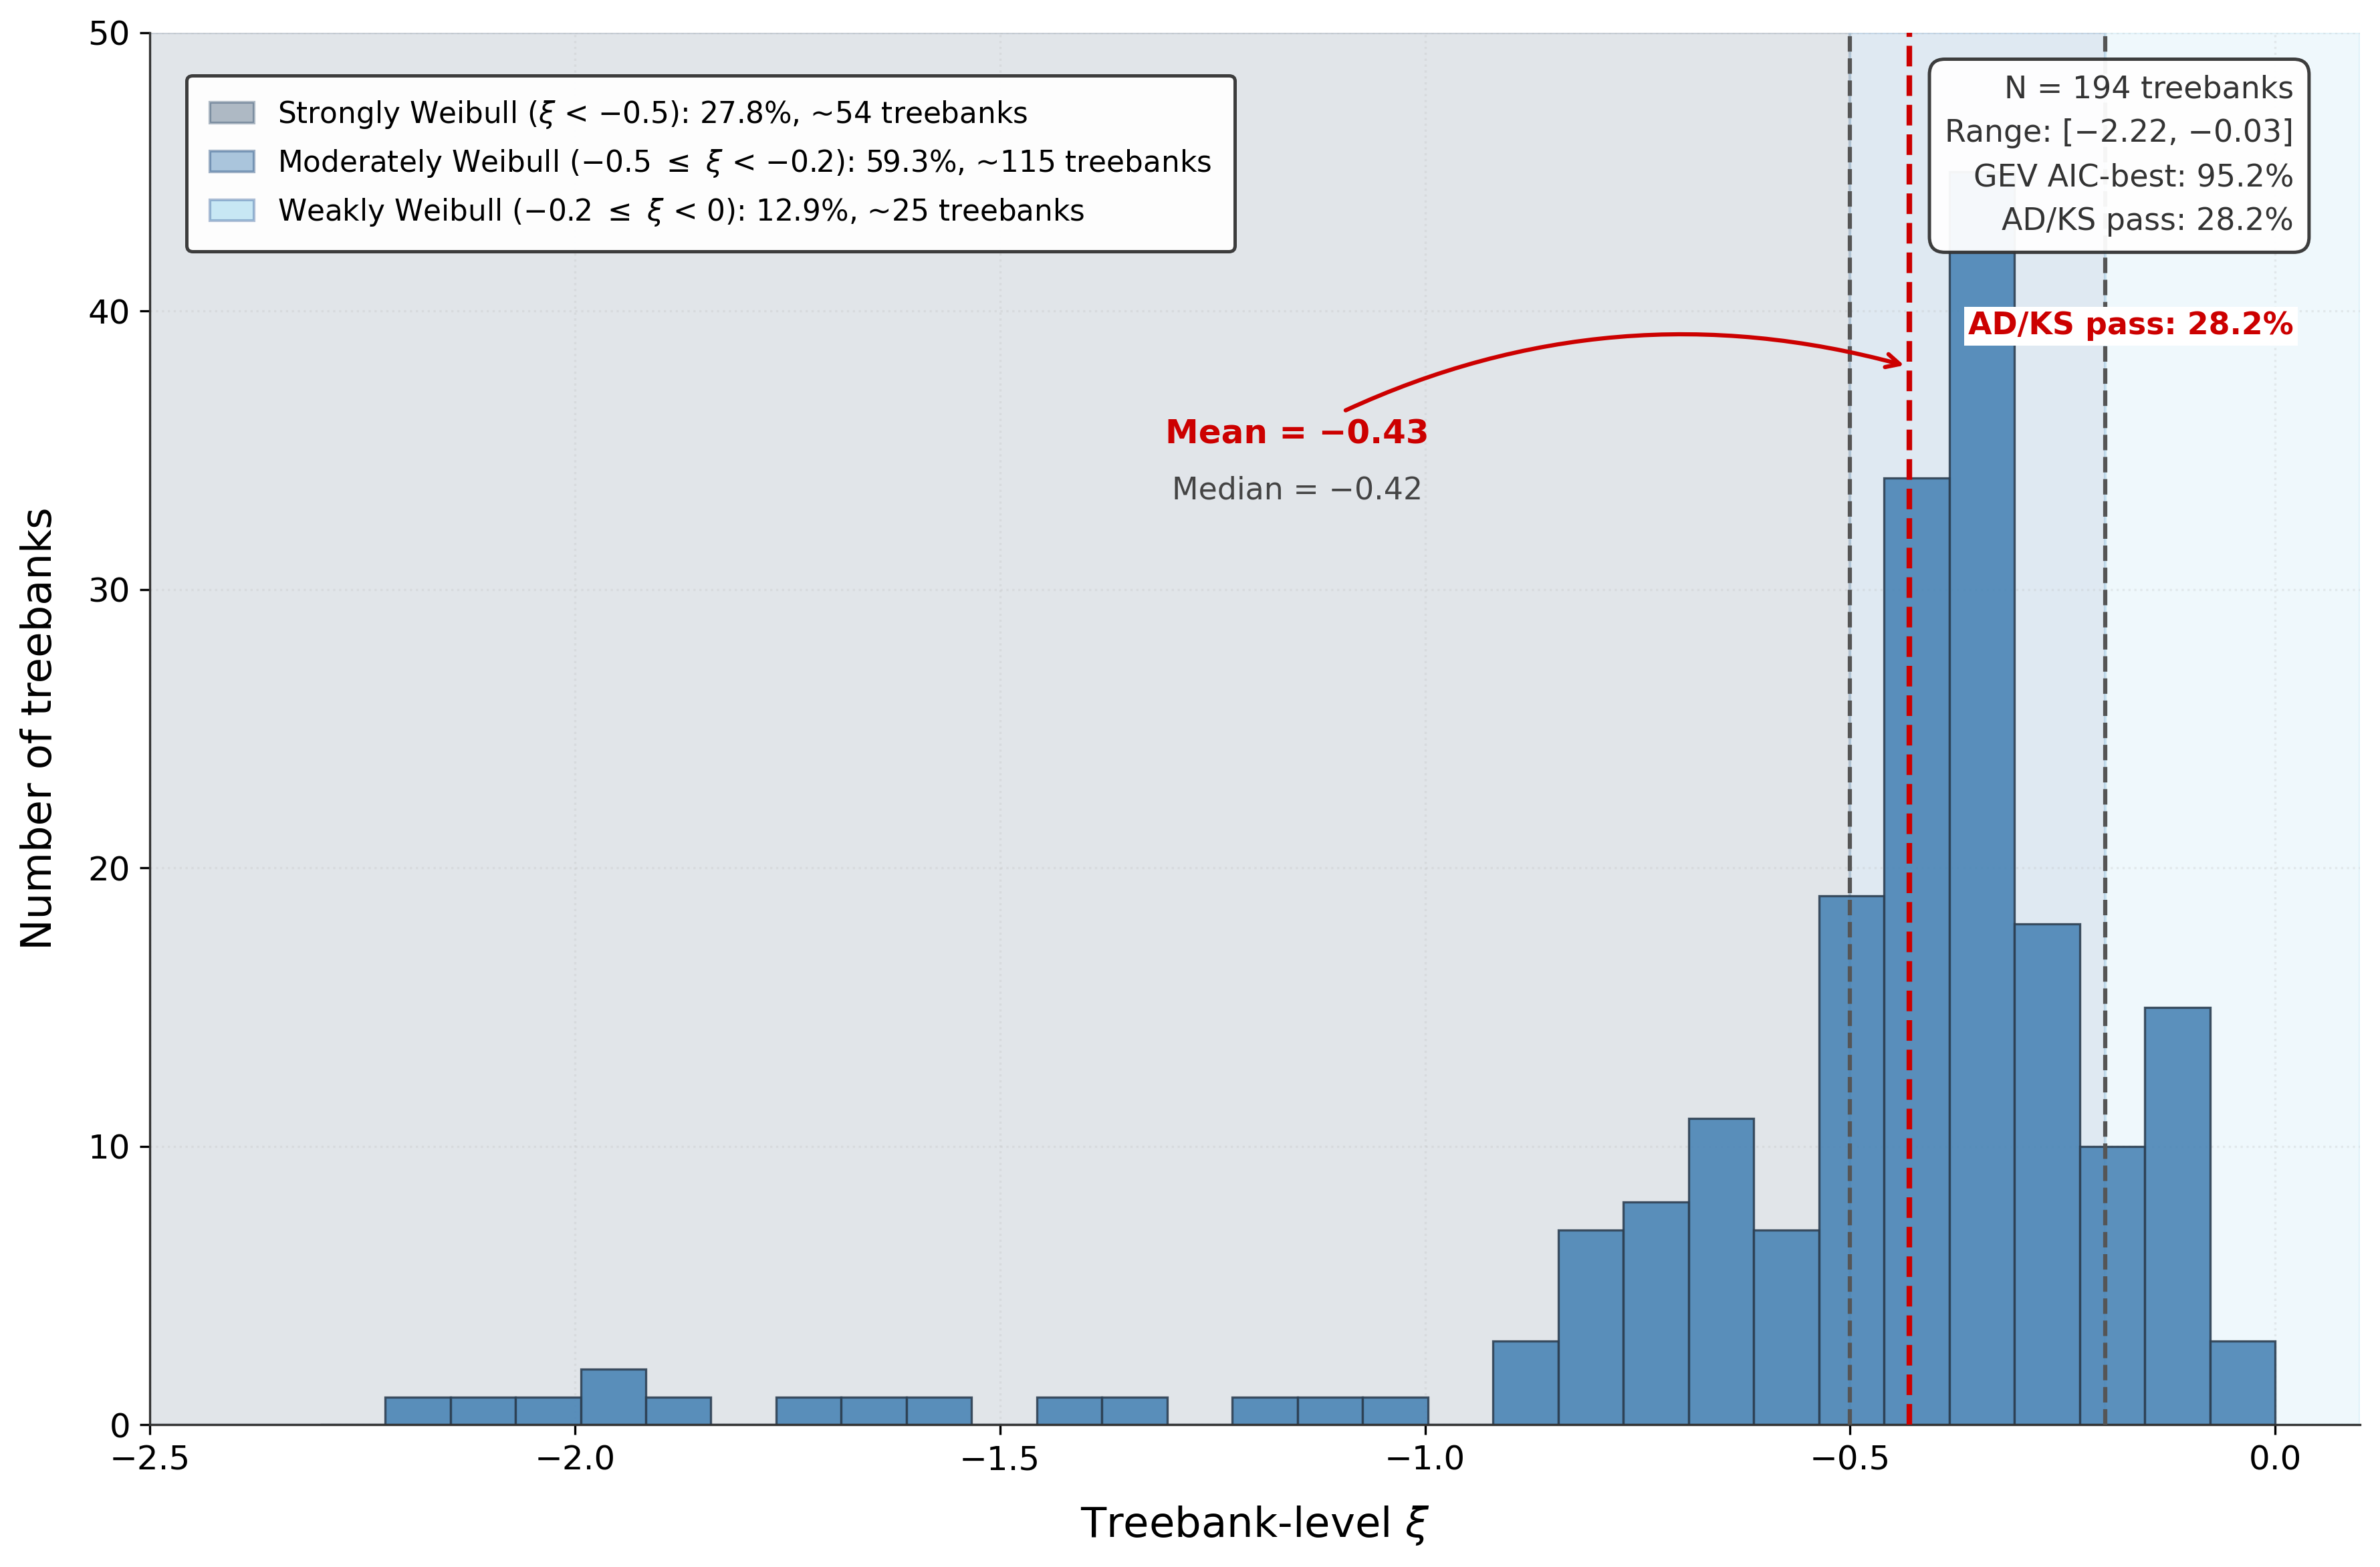
\includegraphics[width=0.75\textwidth,keepaspectratio]{figures/fig2_v0.png}
  \caption{Distribution of treebank-level GEV shape parameter $\xi$ across 194 treebanks (inverse-variance weighted across qualifying bins). All values fall in the Weibull domain ($\xi < 0$). Dashed vertical lines mark regime boundaries. Inset reports both relative fit quality (GEV AIC-best in 95.2\% of 918 combinations) and absolute fit quality (28.2\% pass Anderson-Darling/KS tests).}
  \label{fig:xi_dist}
\end{figure}

\subsection{Bound-Awareness Validation}

The bound-awareness simulation across 10 typologically diverse treebanks at 6 sentence lengths reveals length-dependent results. The null $\xi$ range under random projective linearization increases monotonically with sentence length: 0.15 at $n{=}10$, 0.20 at $n{=}12$, 0.27 at $n{=}14$, 0.30 at $n{=}16$, 0.42 at $n{=}18$, and 0.52 at $n{=}20$. The 0.25 viability threshold is crossed at $n{=}14$, yielding a length-dependent track recommendation: the normalized track is preferred for $n{=}10$ and $n{=}12$ (where bound domination is uniform across treebanks), while the raw track supports meaningful cross-treebank variation for $n \geq 14$.

A uniform-random baseline (integers drawn uniformly from $[1, n{-}1]$ with no tree structure) produces $\xi \approx -0.28$, substantially less negative than the null distribution from random projective linearizations ($\xi$ ranging from $-0.49$ to $-1.04$). This gap confirms that tree structure --- not the theoretical bound alone --- drives the strongly negative null $\xi$ values. These results are summarized in Figure~\ref{fig:bound_awareness}.

\begin{figure}[!htbp]
  \centering
  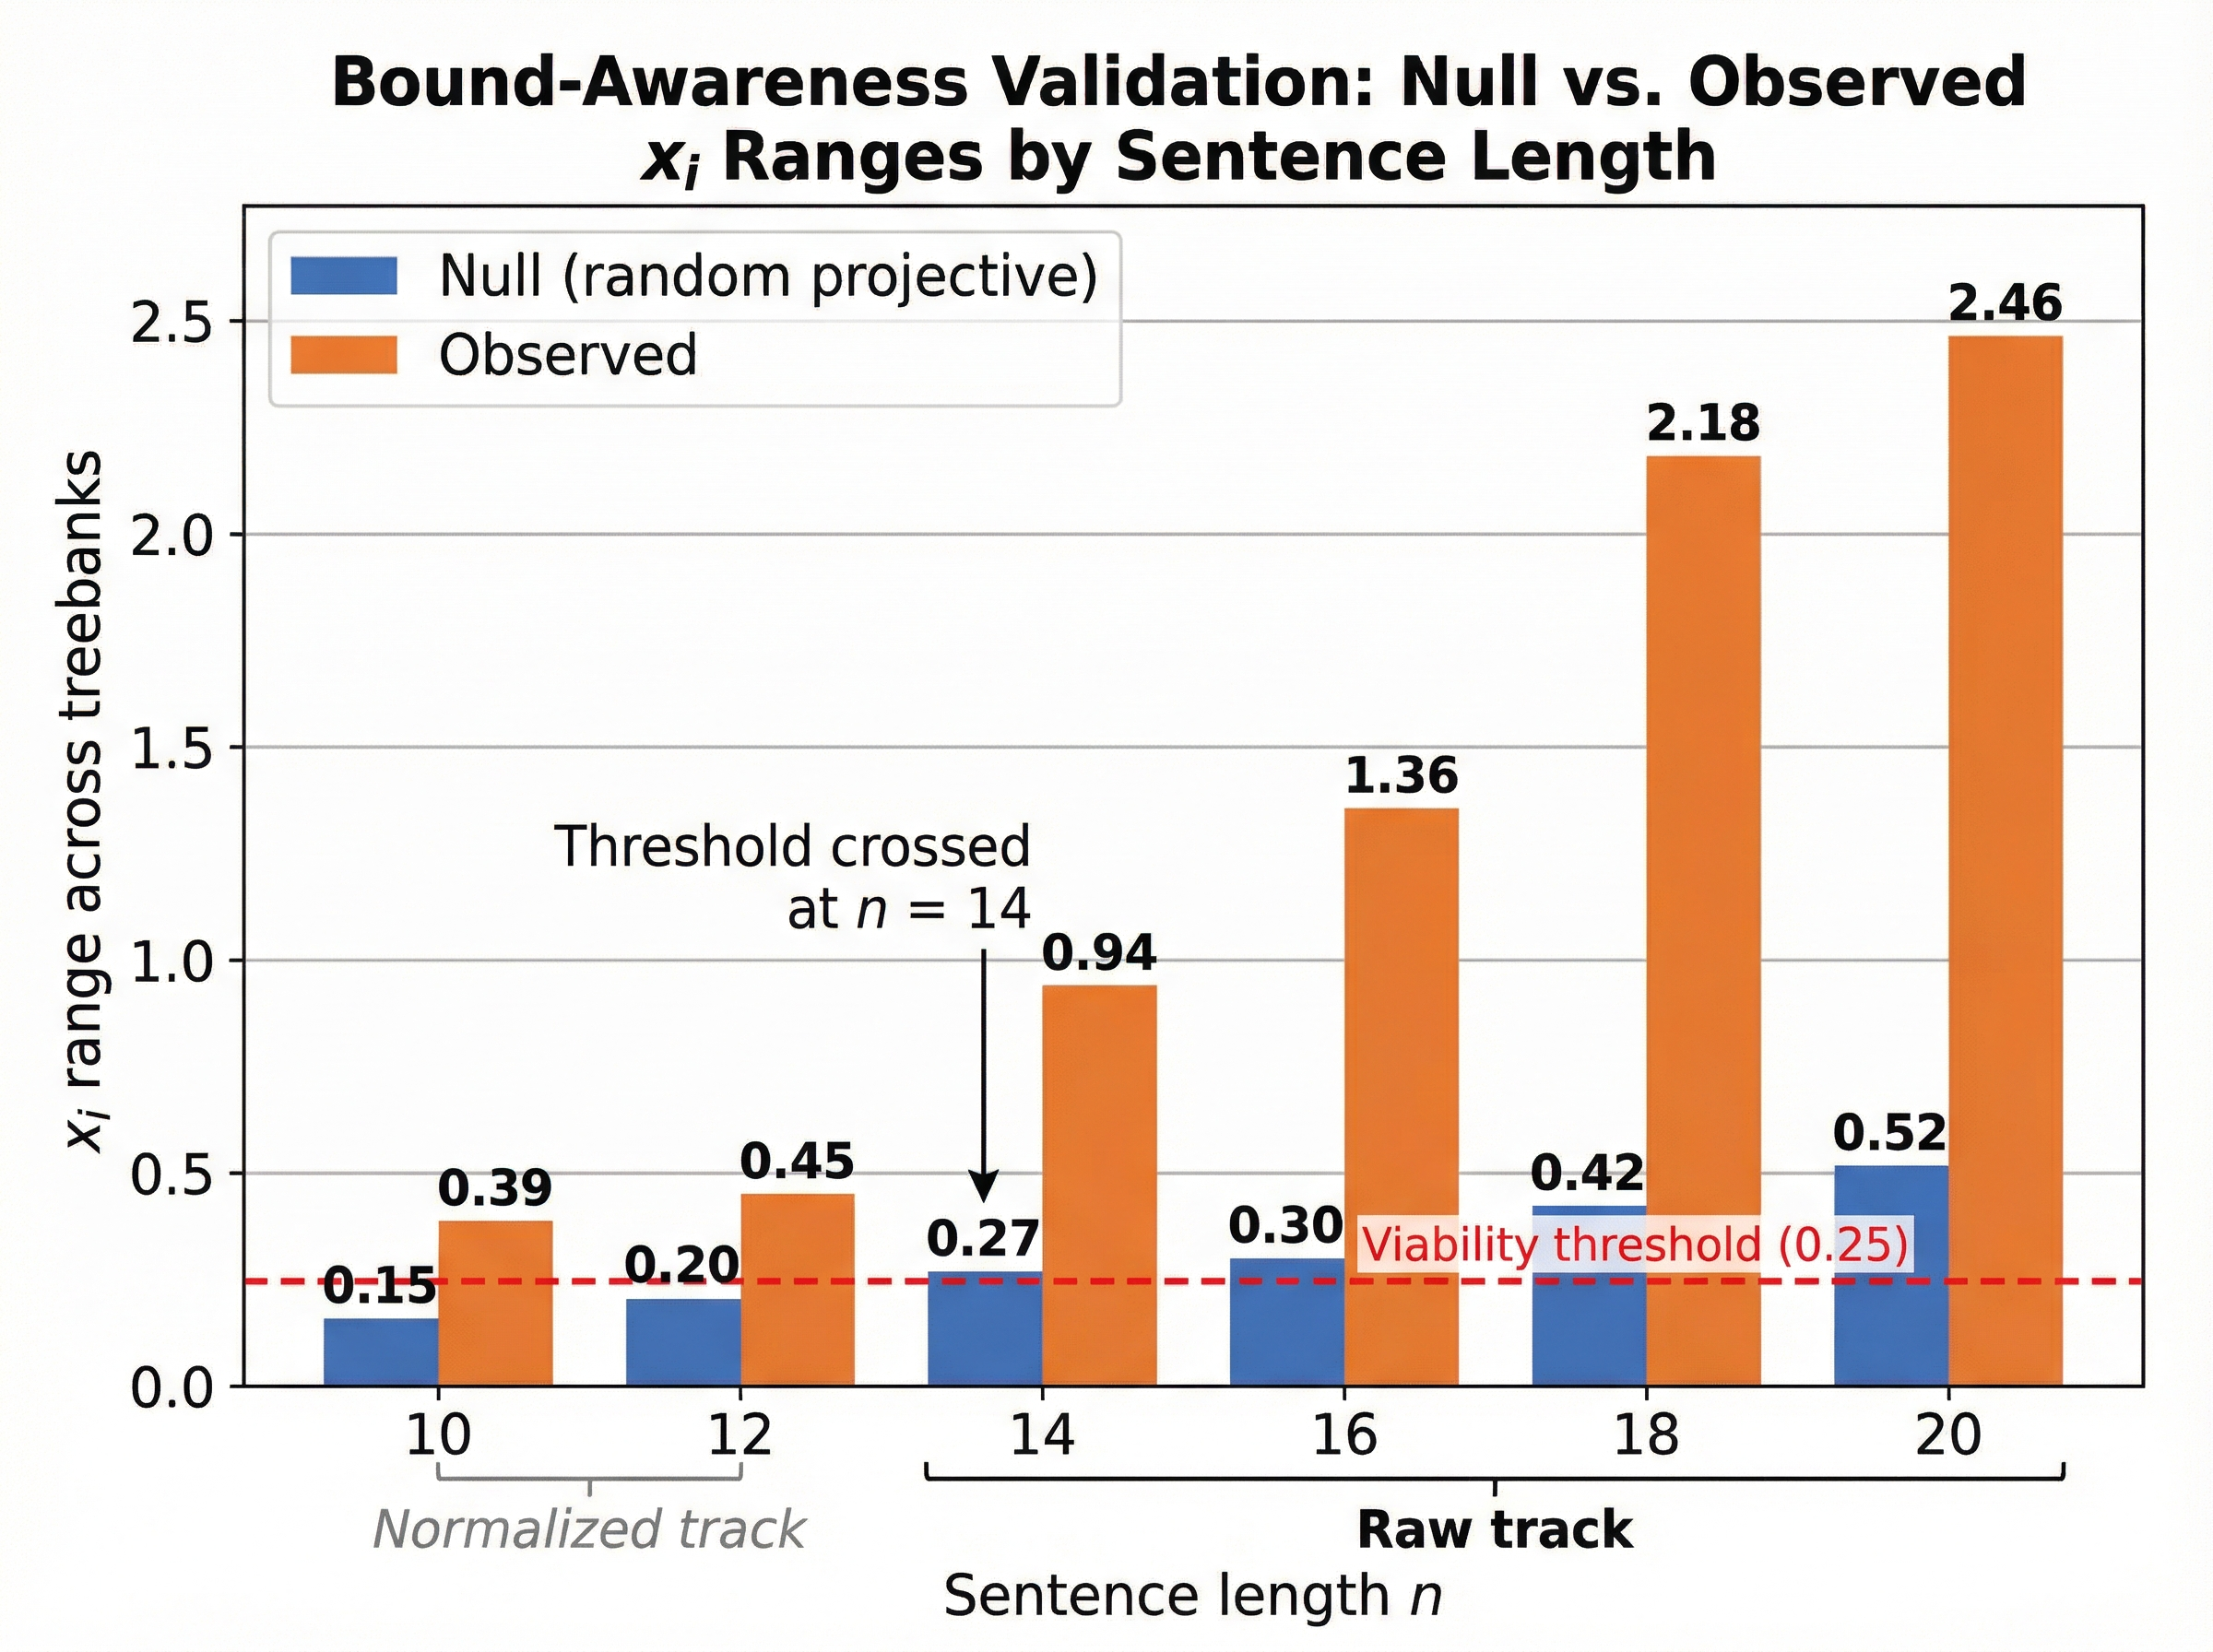
\includegraphics[width=0.80\textwidth,keepaspectratio]{figures/fig3_v0.png}
  \caption{Bound-awareness validation results across six sentence lengths. Blue bars show the range of $\xi$ estimates under the null model (random projective linearization of observed trees); orange bars show the observed $\xi$ range across 10 typologically diverse treebanks. The horizontal dashed line marks the 0.25 viability threshold. For $n \geq 14$, the null $\xi$ range exceeds 0.25, indicating that cross-treebank $\xi$ variation in the raw track reflects genuine structural differences rather than bound proximity alone.}
  \label{fig:bound_awareness}
\end{figure}

\subsection{Dual-Track Agreement}

The raw-track and normalized-track $\xi$ estimates show Spearman $\rho = 0.9997$ ($p < 10^{-307}$) across treebank rankings, far exceeding the 0.8 robustness threshold. This concordance indicates that typological interpretations are robust to the choice of normalization.

\subsection{Super-Block Sensitivity and Ordinal Validity}

The super-block sensitivity analysis reveals a critical negative result: single-sentence and super-block $\xi$ estimates show significant \emph{negative} correlations --- $\rho = -0.39$ ($K = 20$, 95\% CI $[-0.53, -0.24]$), $\rho = -0.55$ ($K = 30$, 95\% CI $[-0.70, -0.36]$) --- with all validation flags set to False. This anti-correlation arises because the max-of-max operation on bounded integer data produces ceiling concentration: 40.7\% of super-block GEV fits yield degenerate $\xi$ estimates. Super-block maxima cluster near the theoretical bound $n{-}1$, collapsing distributional variation and inverting $\xi$ rankings.

Non-parametric quantile comparison reveals near-perfect rank preservation: the 95th-percentile max\_DD values correlate at $\rho = 0.986$ and 99th-percentile values at $\rho = 0.996$ between single-sentence and super-block regimes. These quantile correlations validate that treebanks producing more extreme max\_DD values at the single-sentence level also produce more extreme values at the super-block level. However, quantile rank preservation validates ordinal extremeness of the \emph{data}, not the interpretability of $\xi$ as a tail-shape \emph{parameter}. The anti-correlation of parametric $\xi$ estimates across scales indicates that single-sentence $\xi$ should not be interpreted as a precise measure of tail-decay rate.

A formal ordinal validity evaluation produces mixed results across four tests: bootstrap rank stability yields mean Kendall $\tau = 0.770$ (below the 0.80 threshold); rank regression of $\xi$ on entropy is non-significant ($p = 0.126$); permutation testing yields $p = 0.090$; while simulation recovery of known $\xi$ rankings from synthetic GEV data passes ($\rho = 0.963$). The simulation result confirms that L-moments estimation \emph{can} recover ordinal $\xi$ structure from GEV-distributed data, but the empirical tests suggest that the $\xi$--entropy relationship is not robust at the purely ordinal level. Together, these results support interpreting $\xi$ as an approximate descriptive index rather than a precise ordinal ranking.

\subsection{Typological Regression}

Mixed-effects regression of treebank-level $\xi$ on three standardized typological predictors with 26 language-family random intercepts (172 treebanks with complete data) identifies word-order entropy as the sole significant predictor ($\beta = 0.084$, SE $= 0.023$, $p_{\text{FDR}} = 0.0007$), while morphological richness ($\beta = -0.027$, SE $= 0.022$, $p_{\text{FDR}} = 0.21$) and head-direction ratio ($\beta = -0.031$, SE $= 0.022$, $p_{\text{FDR}} = 0.21$) are non-significant after FDR correction.

All VIFs remain below 1.4, indicating no multicollinearity concerns. The partial correlation of word-order entropy with $\xi$ is $r = 0.246$ ($p = 0.001$), while morphological richness ($r = -0.118$, $p = 0.12$) and head-direction ratio ($r = -0.073$, $p = 0.34$) show no significant partial associations. The model pseudo-$R^2 = 0.164$, meaning that approximately 84\% of cross-treebank $\xi$ variance remains unexplained. Word-order entropy alone achieves pseudo-$R^2 = 0.119$; adding morphological richness and head-direction ratio contributes only 2.6 percentage points of additional explained variance\footnote{Code: \url{https://github.com/AMGrobelnik/ai-invention-42dac1-word-order-entropy-predicts-ordinal-tail/tree/main/evaluation_iter3_honest_mediatio}}. The substantial unexplained variance indicates that additional factors --- genre, corpus size, annotation quality, areal effects, and linguistic properties not captured by the three predictors --- likely contribute substantially to cross-treebank $\xi$ variation.

The positive sign of the word-order entropy coefficient has a clear directional interpretation: languages with freer word order (higher entropy) show less negative $\xi$ --- a softer, less sharply bounded tail constraint --- while languages with rigid word order show more strongly negative $\xi$, indicating sharper upper bounds on extreme dependency distances. This relationship is visualized in Figure~\ref{fig:entropy_xi}.

\begin{figure}[!htbp]
  \centering
  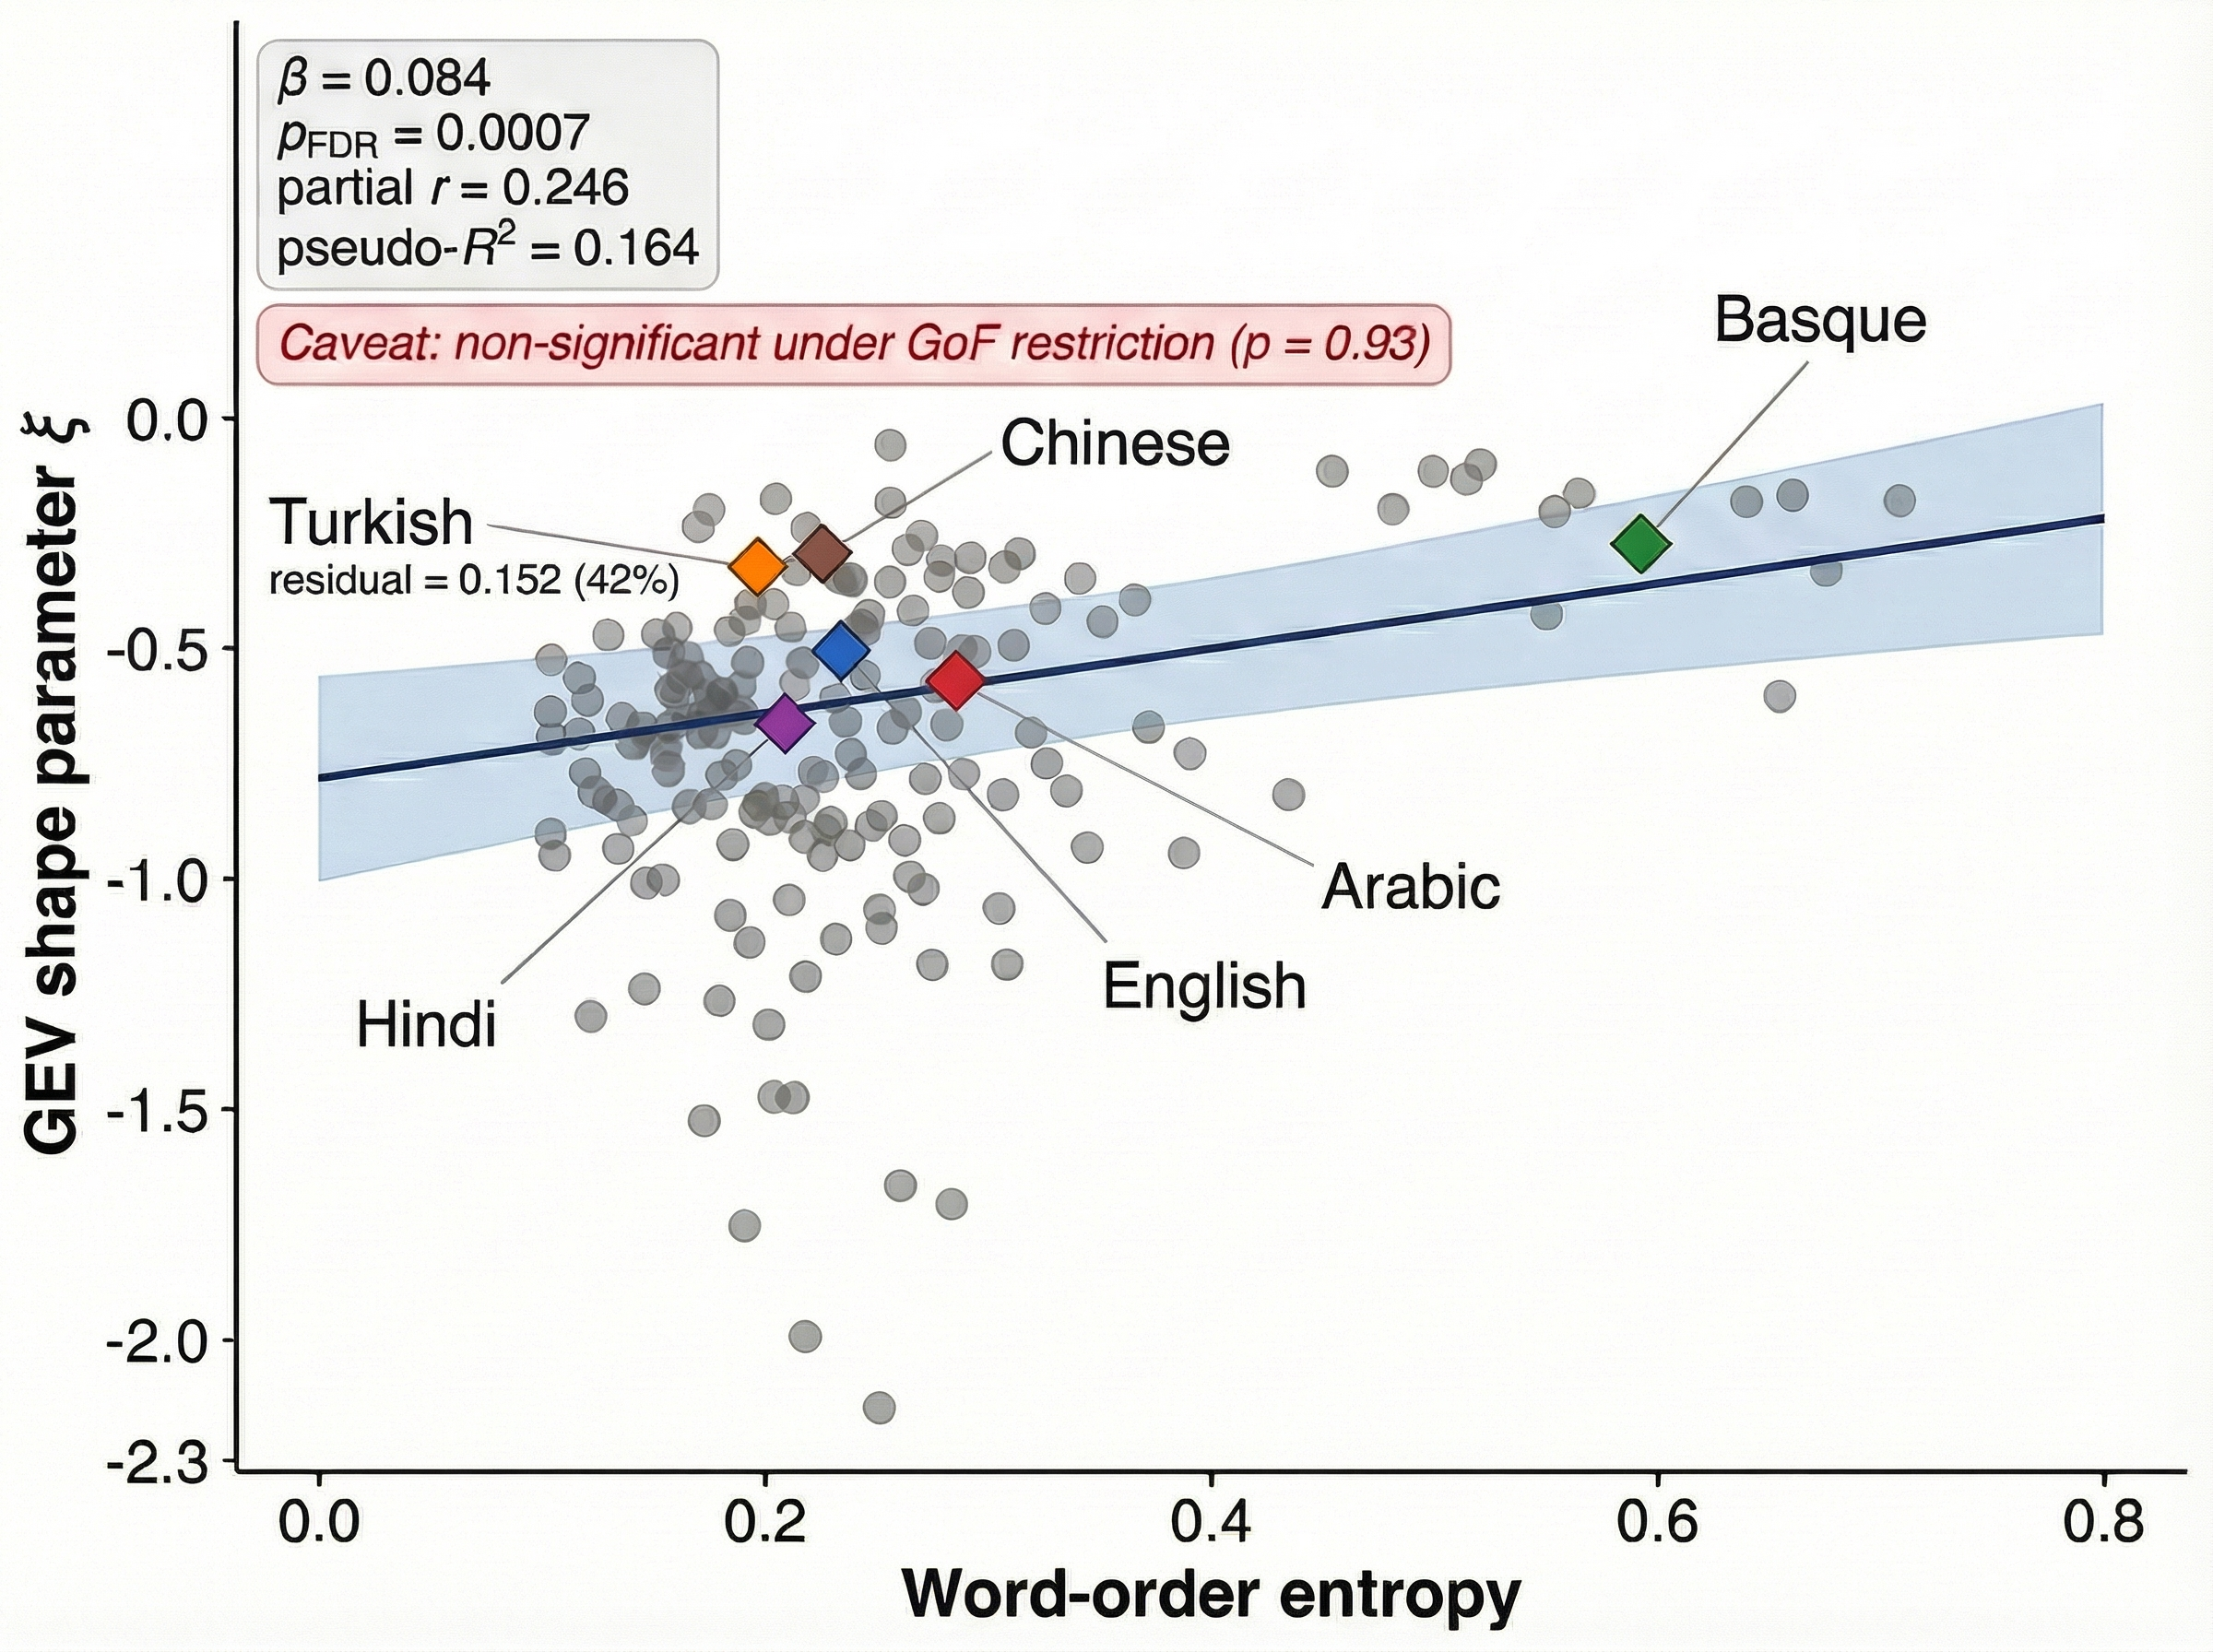
\includegraphics[width=0.80\textwidth,keepaspectratio]{figures/fig4_v0.png}
  \caption{Scatter plot of treebank-level word-order entropy \cite{Levshina2019} against GEV shape parameter $\xi$ for 172 treebanks in the regression sample. The regression line (solid) shows the positive association ($\beta = 0.084$, $p_{\text{FDR}} = 0.0007$, partial $r = 0.246$). Six key languages are annotated. Languages with freer word order (higher entropy) show softer tail constraints (less negative $\xi$). The shaded band indicates the 95\% confidence region. Note: this association vanishes when restricted to GEV fits passing absolute goodness-of-fit ($p = 0.93$; see Section~\ref{sec:sensitivity}).}
  \label{fig:entropy_xi}
\end{figure}

\subsection{Sensitivity Analyses}\label{sec:sensitivity}

The word-order entropy association is tested across four sensitivity tracks:

\textbf{Family-audit correction.} After correcting Afrikaans from Afro-Asiatic to Indo-European, the entropy coefficient changes negligibly ($\beta = 0.0835$ vs.\ $0.084$, confidence intervals fully overlapping). The corrected model is reported as primary throughout.

\textbf{Goodness-of-fit restriction.} When the analysis is restricted to the 259 of 918 combinations (28.2\%) passing the KS goodness-of-fit test, retaining 120 treebanks (104 with complete typological data, 22 families), word-order entropy becomes entirely non-significant ($\beta = -0.014$, $p = 0.47$, $p_{\text{FDR}} = 0.70$). The model pseudo-$R^2$ drops to 0.065. This result means the entropy--$\xi$ association observed in the full sample depends on $\xi$ estimates from GEV fits that fail absolute goodness-of-fit --- a finding that substantially qualifies the typological interpretation. Two interpretations are possible: (a) the GEV captures ordinal information about tail constraints even when the parametric form does not perfectly describe the distribution, or (b) systematic biases in poorly-fitting $\xi$ estimates happen to correlate with word-order entropy. The present data cannot distinguish these alternatives.

\textbf{Annotation-quality filtering.} Restricting to 131 treebanks with feature-annotation completeness above 0.5 (20 families), the entropy coefficient is attenuated but remains significant at the $p < 0.05$ level ($\beta = 0.047$, SE $= 0.018$, $p = 0.009$, $p_{\text{FDR}} = 0.028$). The reduced coefficient magnitude (0.047 vs.\ 0.084) suggests that annotation-quality variation inflates the entropy effect in the full sample, but does not entirely account for the association. The annotation completeness--morphological richness confound ($\rho = 0.79$) is attenuated to $\rho = 0.41$ in the filtered subset.

\textbf{Leave-one-family-out.} Across 26 family-drop iterations, the mean entropy coefficient is $\beta = 0.084$ (SD $= 0.012$), with 92.3\% (24 of 26) yielding significant results. The most influential family is Tucanoan ($\beta$ drops to 0.040), and Indo-European removal produces the highest coefficient ($\beta = 0.123$). No single language family drives the association.

In summary, the entropy--$\xi$ association is robust to genealogical correction, annotation filtering, and family-level influence, but is not robust to restriction to well-fitting GEV combinations. The primary finding should be interpreted as suggestive evidence for a word-order entropy association, qualified by its dependence on the full set of GEV fits.

\subsection{Mediation Analysis}

The Preacher--Hayes mediation analysis (5,000 bootstrap resamples) tests whether word-order entropy mediates the morphology $\rightarrow \xi$ pathway. The results reveal a classical suppression pattern with opposing paths:

\begin{itemize}
  \item \textbf{Indirect effect} (morphology $\rightarrow$ entropy $\rightarrow \xi$): $0.029$, 95\% CI $[0.009, 0.055]$, significant.
  \item \textbf{Direct effect} (morphology $\rightarrow \xi$, controlling for entropy): $-0.026$, 95\% CI $[-0.057, 0.001]$, non-significant.
  \item \textbf{Total effect}: $0.002$, near zero.
\end{itemize}

The near-zero total effect arises because the positive indirect path ($+0.029$) and negative direct path ($-0.026$) nearly cancel. The proportion mediated (indirect/total $= 11.78$) is nonsensical in the presence of opposing paths and should not be interpreted as indicating that 1,178\% of the effect is mediated. Rather, morphological richness has effectively no net association with $\xi$; the indirect and direct paths represent opposing statistical tendencies that sum to approximately zero.

This pattern is statistically consistent with a structural-distributional interpretation --- richer morphology associates with freer word order, which associates with softer tail constraints --- but the cross-sectional design cannot establish the causal ordering. As Maxwell and Cole \cite{Maxwell2007} demonstrated, cross-sectional mediation typically generates biased estimates of longitudinal parameters even under ideal conditions. Alternative causal models, including reverse mediation (entropy $\rightarrow$ morphology $\rightarrow \xi$) and common-cause confounding, cannot be ruled out on statistical grounds alone.

However, a reverse mediation analysis provides one asymmetric piece of evidence: the reverse indirect path (entropy $\rightarrow$ morphology $\rightarrow \xi$) is non-significant ($-0.010$, 95\% CI $[-0.025, 0.002]$), while the forward indirect path is significant. The forward and reverse models are thus statistically distinguishable, providing weak evidence favoring the forward direction. The full mediation path diagram is shown in Figure~\ref{fig:mediation}.

When restricted to well-annotated treebanks (feature completeness $> 0.5$, 135 treebanks, 19 families), the opposing-path pattern does not persist: the total effect becomes positive ($0.034$), the indirect path remains significant ($0.016$, CI $[0.003, 0.032]$), and the direct path remains non-significant ($0.018$, CI $[-0.014, 0.049]$). The disappearance of the suppression pattern suggests that annotation-quality variation contributes to the opposing paths observed in the full sample.

\begin{figure}[!htbp]
  \centering
  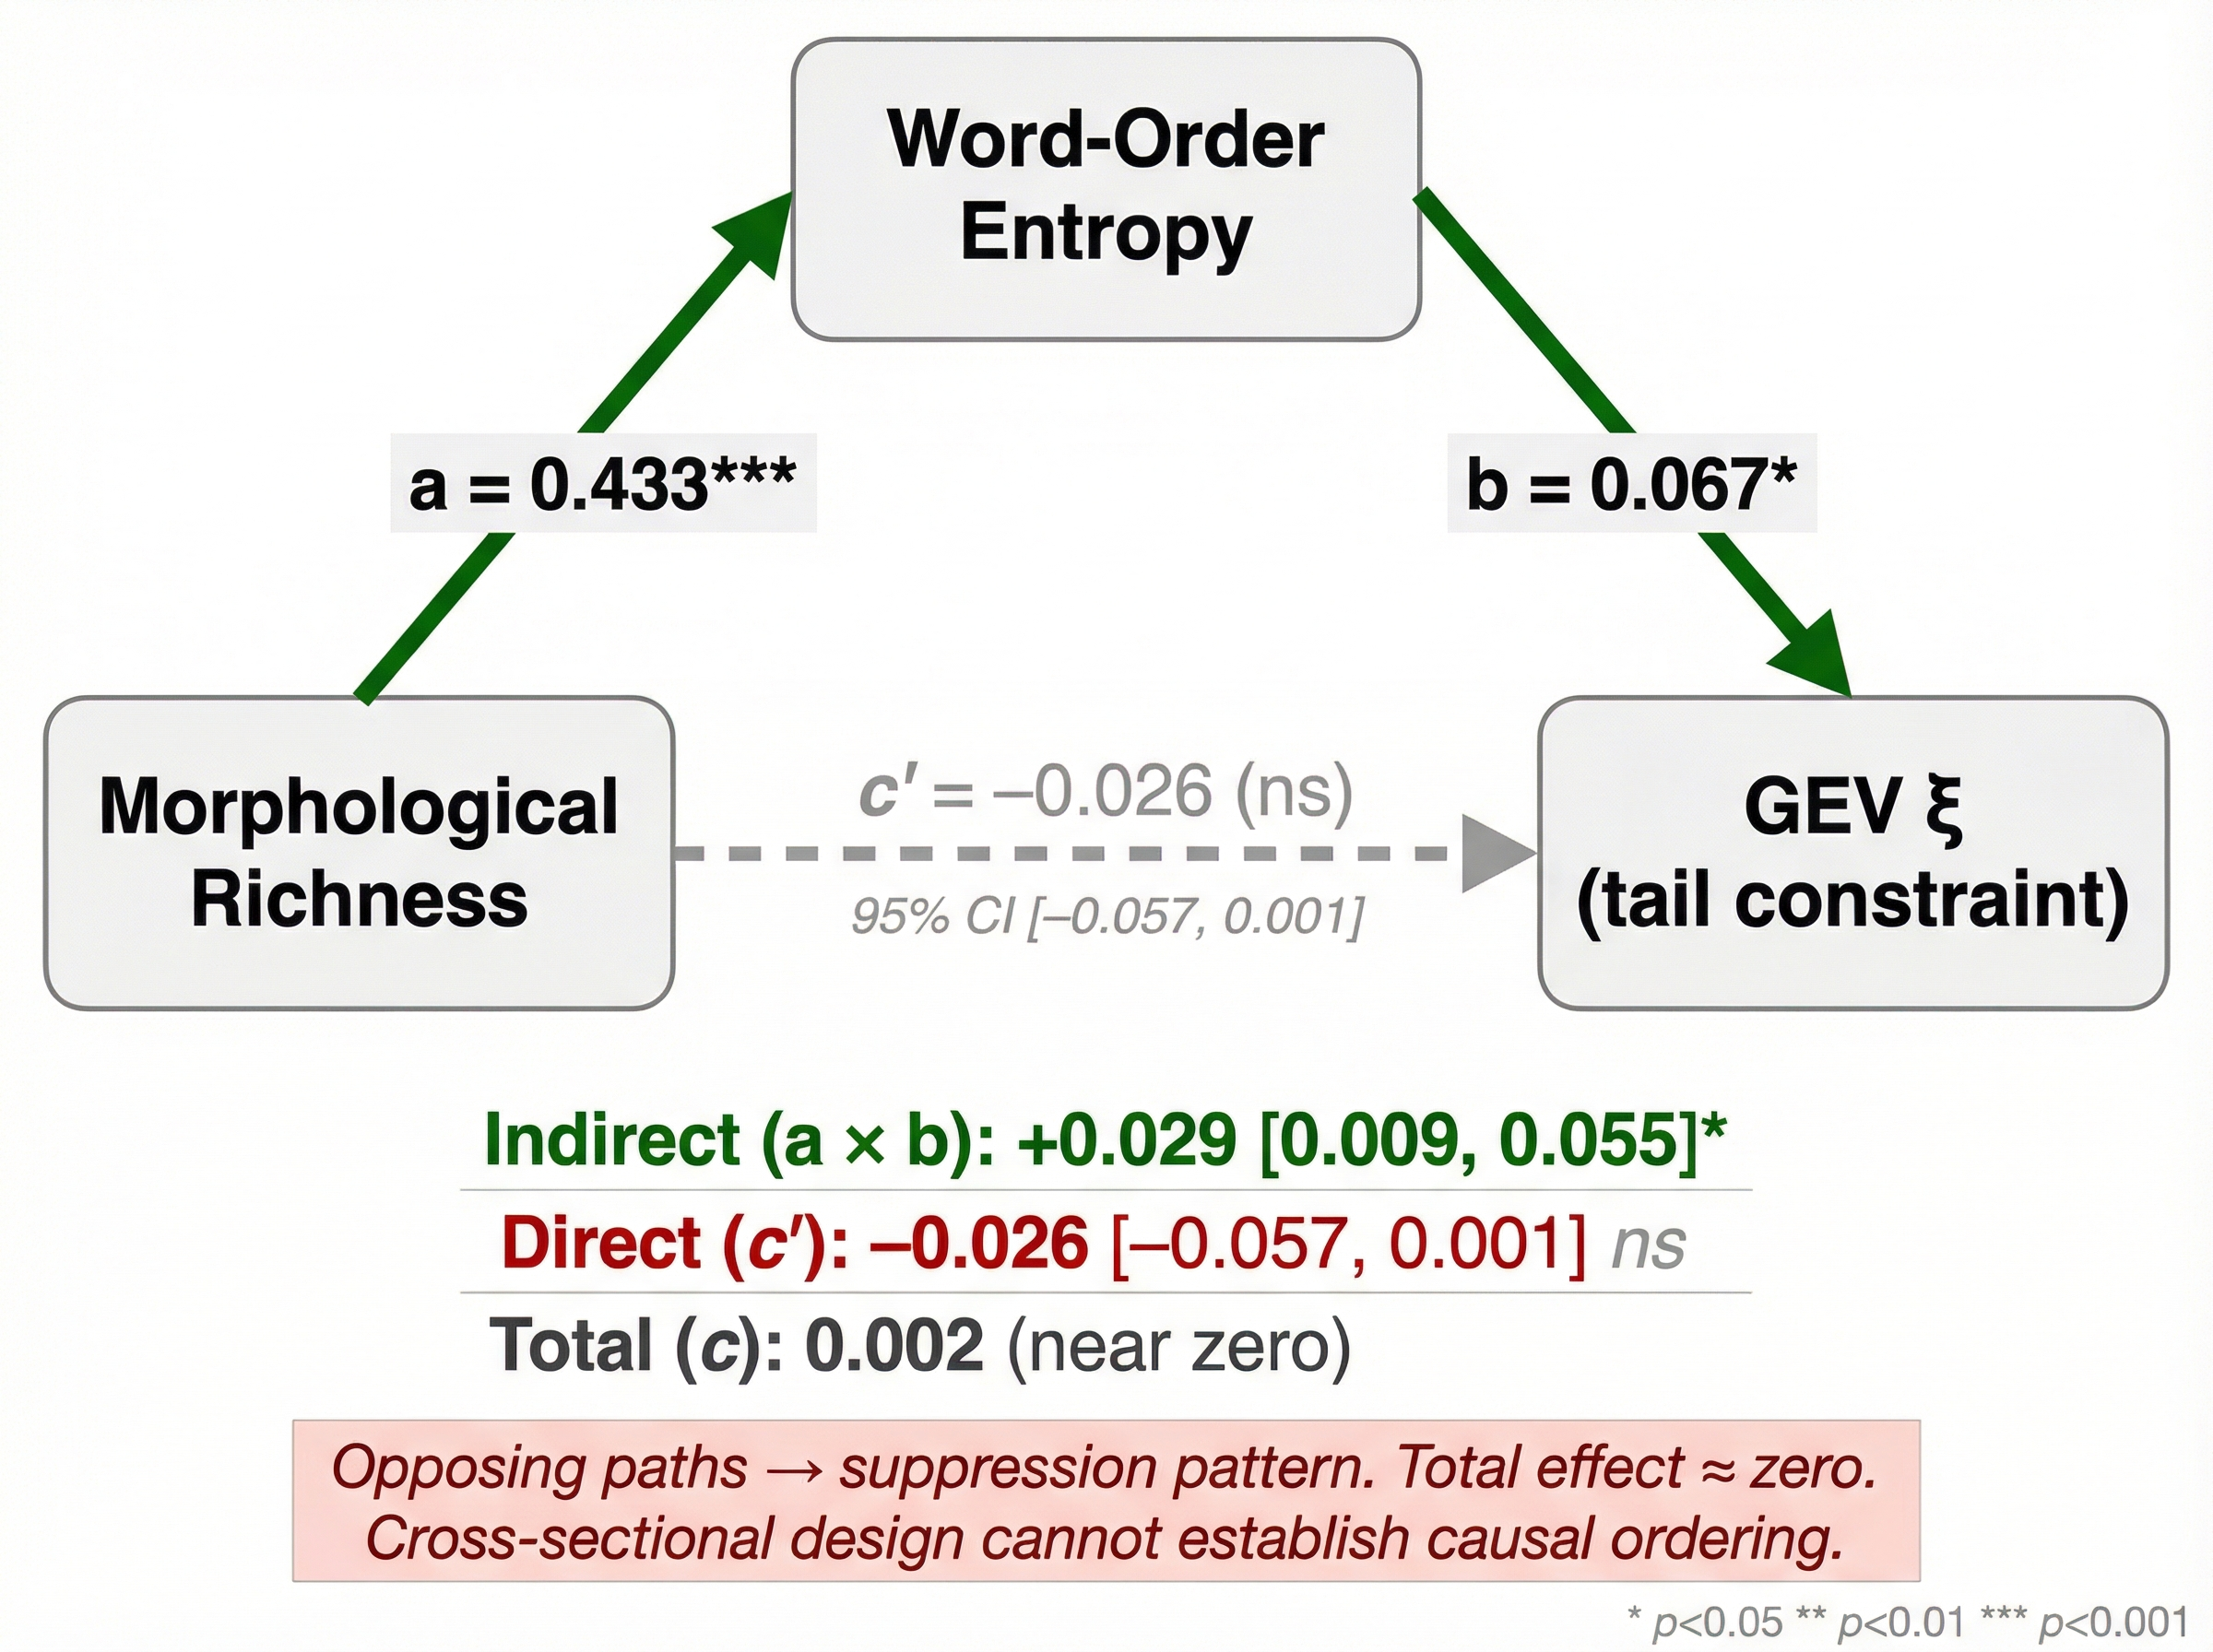
\includegraphics[width=0.80\textwidth,keepaspectratio]{figures/fig5_v0.png}
  \caption{Mediation analysis of the morphological richness $\rightarrow$ word-order entropy $\rightarrow$ $\xi$ pathway (Preacher--Hayes bootstrap, 5,000 resamples). The indirect path ($a \times b = 0.029$) is significant, but the direct path ($c' = -0.026$) opposes it, yielding a near-zero total effect ($c = 0.002$). The opposing paths represent a classical suppression pattern; cross-sectional mediation cannot establish causal ordering \cite{Maxwell2007}. Solid arrows indicate significant paths; dashed arrows indicate non-significant paths.}
  \label{fig:mediation}
\end{figure}

\subsection{EVT-Unique Information}

A systematic analysis quantifies the added value of GEV tail parameters over mean dependency distance. Among 18,721 pairwise treebank comparisons, 9,410 pairs have similar mean DD (within threshold). Of these, 4,352 pairs (46.2\%) differ meaningfully in $\xi$, far exceeding the 20\% threshold for demonstrating systematic added value. This result confirms that $\xi$ captures a dimension of cross-linguistic variation orthogonal to mean dependency distance --- the framework's most robust empirical contribution, which does not depend on any specific typological predictor.

\subsection{Discordant Language Profiles}

The discordant language profiles provide targeted illustrations of the word-order entropy association. Basque (eu\_bdt) --- morphologically rich (1.99) with high word-order entropy (0.586) --- exhibits $\xi = -0.347$, a relatively soft tail constraint consistent with its high entropy. Hindi (hi\_hdtb) --- also morphologically rich (2.89) but with low entropy (0.210) --- shows $\xi = -0.634$, one of the most strongly bounded tails. Both languages are morphologically rich, but their $\xi$ values diverge in the direction predicted by word-order entropy. Arabic (ar\_padt), with rich morphology (2.38) and a head-initial profile (HDR $= 0.686$) but low entropy (0.262), shows $\xi = -0.574$ --- aligning with its rigid word order rather than its rich morphology.

Turkish (tr\_imst) presents a case where the model underperforms: despite rich morphology (2.75) and low entropy (0.193), Turkish shows $\xi = -0.365$ --- substantially less negative than the model predicts (predicted $\xi = -0.517$, residual $= 0.152$, representing 42\% of its $\xi$ value). Turkish's agglutinative morphology may enable long-distance dependencies through mechanisms not captured by the three predictors --- transparent morpheme boundaries and predictable suffixation patterns that reduce working-memory load at long distances. The mean absolute residual across all treebanks is 0.147 (median $= 0.106$), confirming that while the model captures the central tendency, individual predictions carry substantial uncertainty.

\subsection{Spoken/Written Comparison}

Two spoken/written treebank pairs are available after excluding the domain-restricted en\_atis corpus (Air Travel Information System), which consists of formulaic airline booking queries rather than natural spoken language. In both remaining pairs, spoken treebanks show less negative $\xi$ (softer constraint) than written counterparts: Slovenian (spoken $\xi = -0.331$ vs.\ written $\xi = -0.387$, Cohen's $d = 2.74$, 95\% CI $[2.34, 3.21]$) and French (spoken $\xi = -0.303$ vs.\ written $\xi = -0.424$, $d = 5.01$, 95\% CI $[4.17, 5.85]$). The consistent direction suggests that editorial processes in written language constrain extreme dependencies more tightly than real-time spoken production, where shorter planning horizons may permit occasional very long dependencies. The sample of two pairs is too small for generalization; additional spoken treebanks are needed to confirm this pattern.

\subsection{Genre Control}

Within-language $\xi$ variation across genres provides context for interpreting the typological effects. English ranges from $\xi = -0.517$ (en\_ewt) to $-0.344$ (en\_partut), a within-language range of 0.173. Italian shows the largest range at 0.211 (it\_partut $-0.271$ to it\_vit $-0.481$), while French shows near-perfect stability (range $= 0.007$). The cross-language standard deviation of $\xi$ (0.228) exceeds the mean within-language genre variation, indicating that the typological signal is not dominated by genre confounds, though genre contributes non-negligible variation within individual languages.

\section{Discussion}\label{sec:discussion}

\subsection{The GEV Framework: What It Captures and What It Cannot}

The primary contribution of this work is introducing an EVT framework for characterizing the tail behavior of maximum dependency distances, together with validation protocols that honestly assess its applicability to bounded linguistic data. The framework succeeds at demonstrating that tail-constraint severity varies substantially across languages and that this variation is orthogonal to mean dependency distance (46.2\% of similar-mean pairs differ in $\xi$). The dual-track design achieves near-perfect agreement ($\rho = 0.9997$), confirming robustness to normalization choice.

The framework's limitations are equally important. The low absolute goodness-of-fit rate (28.2\%) means that GEV provides a poor parametric description of max\_DD distributions in most bins, even though no standard alternative fits better. The super-block sensitivity analysis reveals negative $\xi$ correlations across scales ($\rho = -0.39$ to $-0.55$), arising from ceiling concentration in bounded integer data, and the formal ordinal validity evaluation produces mixed results (1 of 4 tests pass). Together, these findings indicate that $\xi$ should be treated as an approximate descriptive index of tail-constraint severity, not as a precise estimate of the asymptotic tail-decay regime. The three-regime GEV classification (Weibull/Gumbel/Fr\'echet) is not supported by these data; the entire sample falls in the Weibull domain, and the meaningful variation is in the gradient from strongly to weakly negative $\xi$.

\subsection{Word-Order Entropy: Genuine Signal or Artifact?}

The regression identifies word-order entropy as the sole significant predictor of $\xi$ ($\beta = 0.084$, $p_{\text{FDR}} = 0.0007$), with a clear directional interpretation: languages with freer word order show softer tail constraints. The association is robust to family-audit correction ($\beta = 0.0835$), annotation-quality filtering ($\beta = 0.047$, $p = 0.009$), and leave-one-family-out cross-validation (92.3\% significant across 26 drops). These tests address genealogical non-independence, annotation artifacts, and individual-family leverage, respectively.

However, the association vanishes entirely when analysis is restricted to GEV fits passing absolute goodness-of-fit tests ($\beta = -0.014$, $p = 0.93$). This null result under GoF restriction is the most important qualification of the typological finding. The entropy--$\xi$ association in the full sample may reflect systematic patterns in how GEV misfits vary with typological properties, rather than a genuine relationship between word-order flexibility and tail-constraint severity. Alternatively, the GoF-restricted subset may simply lack statistical power: it retains only 104 treebanks across 22 families, with reduced typological diversity. Resolving this ambiguity requires future work with distributional families better suited to bounded integer data, or substantially larger treebanks where absolute fit may improve.

The model pseudo-$R^2$ of 0.164, while exceeding the baseline mean-DD regression ($R^2 = 0.048$) by over three-fold, leaves approximately 84\% of $\xi$ variance unexplained. Residual analysis reveals no significant associations with corpus size ($r = -0.023$, $p = 0.76$), annotation completeness ($r = -0.10$, $p = 0.18$), or number of binned sentences ($r = -0.11$, $p = 0.16$), and the cumulative additional $R^2$ from all measured confounds is only 0.035. The large unexplained variance likely reflects areal effects, language contact, genealogical inertia, genre composition, and linguistic properties not captured by the three predictors. Turkish's large residual (42\% of its $\xi$) suggests that agglutinative morphology may enable long-distance dependencies through mechanisms that word-order entropy does not capture.

\subsection{Mediation: Consistent With, Not Proving}

The mediation analysis reveals a pattern statistically consistent with the structural-distributional interpretation --- morphological richness associates with $\xi$ through word-order entropy --- but several features of the result warrant cautious interpretation. The near-zero total effect (0.002) means morphological richness has no net association with $\xi$; the indirect and direct paths represent opposing tendencies that cancel. The suppression pattern disappears when annotation-quality confounding is reduced (restricted total effect $= 0.034$), suggesting it is partly artifactual. The reverse mediation model is distinguishable from the forward model (reverse indirect non-significant), providing one asymmetric piece of evidence, but cross-sectional data fundamentally cannot establish causal ordering \cite{Maxwell2007}.

The most defensible conclusion is that word-order entropy --- not morphological richness --- is the relevant typological correlate of $\xi$. The mediation framework reveals the statistical structure of the morphology--entropy--$\xi$ relationships without establishing a causal pathway. Future work with diachronic data (e.g., historical treebanks capturing word-order changes) or controlled experimental paradigms could provide the temporal precedence necessary for causal inference.

\subsection{Implications for Psycholinguistic Theory}

If the association between word-order entropy and $\xi$ reflects a genuine linguistic pattern rather than a statistical artifact of GEV misfit, the structural interpretation has important implications. Rigid-order languages (English, Hindi) mechanically constrain the set of possible word orders, limiting how extreme max\_DD can be, while flexible-order languages (Basque, Czech) permit occasional departures from optimal short-dependency configurations. The constraint on extreme dependency distances would then be a byproduct of word-order rigidity rather than a direct cognitive limitation.

The spoken/written comparison adds a consistent observation: spoken treebanks show softer constraints ($d = 2.74$--$5.01$) than their written counterparts, suggesting that editorial revision in written language imposes tighter bounds on extreme dependencies than real-time spoken production. The sample of two pairs is too small for firm conclusions, but the pattern is consistent with the structural interpretation: written language undergoes additional word-order optimization that spoken language does not.

\section{Conclusion}

This paper introduces an Extreme Value Theory framework for characterizing the tail behavior of maximum dependency distances across 238 Universal Dependencies treebanks spanning 122 languages. By fitting GEV distributions to 918 bin--treebank combinations and extracting the shape parameter $\xi$, the framework reveals cross-linguistic variation invisible to mean-based approaches: 46.2\% of treebank pairs with similar mean dependency distances differ meaningfully in tail-constraint severity.

The typological analysis identifies word-order entropy as a significant correlate of $\xi$ ($\beta = 0.084$, $p_{\text{FDR}} = 0.0007$) that is robust to genealogical correction, annotation-quality filtering, and leave-one-family-out cross-validation, but contingent on including GEV fits that fail absolute goodness-of-fit tests. The mediation analysis reveals a pattern consistent with the structural-distributional interpretation, though opposing indirect and direct paths, a near-zero total effect, and the fundamental limitations of cross-sectional data prevent causal conclusions.

Three methodological innovations --- the bound-awareness simulation protocol, dual-track normalization, and super-block sensitivity analysis --- address fundamental challenges of applying EVT to bounded linguistic data. These protocols revealed important limitations: the GEV parametric form fails absolute fit tests in 72\% of bins, and $\xi$ estimates show negative correlations across block-size scales. The framework works best as a descriptive tool for capturing distributional variation, not as a precise tail-shape estimator for bounded integer data.

Future work should explore distributional families designed for bounded support (e.g., beta-type distributions), extend the framework to other syntactic extremes such as maximum clause depth and maximum filler--gap distance, and apply hierarchical Bayesian GEV models that share information across typologically similar languages. Diachronic applications using historical treebanks could provide the temporal precedence necessary to evaluate causal claims about word-order entropy and processing constraints.

\bibliographystyle{unsrtnat}
\bibliography{references}

\end{document}
